\documentclass[10pt,twocolumn]{article}
% Shared two-column preamble for the three research papers.
% Use with: \documentclass[10pt,twocolumn]{article}
% Then in main.tex: % Shared two-column preamble for the three research papers.
% Use with: \documentclass[10pt,twocolumn]{article}
% Then in main.tex: % Shared two-column preamble for the three research papers.
% Use with: \documentclass[10pt,twocolumn]{article}
% Then in main.tex: \input{../../shared/latex/twocolumn_preamble.tex}

\usepackage[margin=0.75in]{geometry}
\usepackage[utf8]{inputenc}
\usepackage[T1]{fontenc}
\usepackage{lmodern}
\usepackage{microtype}
\usepackage{amsmath,amssymb,amsthm}
\usepackage{graphicx}
\usepackage{booktabs}
\usepackage{caption}
\usepackage{subcaption}
\usepackage{hyperref}
\usepackage{url}
\usepackage{xcolor}
\usepackage{algorithm}
\usepackage{algorithmic}
\usepackage{multirow}
\usepackage{titlesec}
\usepackage{authblk}

\hypersetup{colorlinks=true,linkcolor=blue!50!black,citecolor=blue!50!black,urlcolor=blue!50!black}

\titleformat{\section}{\normalfont\large\bfseries}{\thesection}{0.6em}{}
\titleformat{\subsection}{\normalfont\bfseries}{\thesubsection}{0.5em}{}

\captionsetup{font=small,labelfont=bf,skip=4pt}
\setlength{\columnsep}{0.25in}
\setlength{\parskip}{2pt}

\newtheorem{theorem}{Theorem}
\newtheorem{proposition}[theorem]{Proposition}
\newtheorem{definition}[theorem]{Definition}


\usepackage[margin=0.75in]{geometry}
\usepackage[utf8]{inputenc}
\usepackage[T1]{fontenc}
\usepackage{lmodern}
\usepackage{microtype}
\usepackage{amsmath,amssymb,amsthm}
\usepackage{graphicx}
\usepackage{booktabs}
\usepackage{caption}
\usepackage{subcaption}
\usepackage{hyperref}
\usepackage{url}
\usepackage{xcolor}
\usepackage{algorithm}
\usepackage{algorithmic}
\usepackage{multirow}
\usepackage{titlesec}
\usepackage{authblk}

\hypersetup{colorlinks=true,linkcolor=blue!50!black,citecolor=blue!50!black,urlcolor=blue!50!black}

\titleformat{\section}{\normalfont\large\bfseries}{\thesection}{0.6em}{}
\titleformat{\subsection}{\normalfont\bfseries}{\thesubsection}{0.5em}{}

\captionsetup{font=small,labelfont=bf,skip=4pt}
\setlength{\columnsep}{0.25in}
\setlength{\parskip}{2pt}

\newtheorem{theorem}{Theorem}
\newtheorem{proposition}[theorem]{Proposition}
\newtheorem{definition}[theorem]{Definition}


\usepackage[margin=0.75in]{geometry}
\usepackage[utf8]{inputenc}
\usepackage[T1]{fontenc}
\usepackage{lmodern}
\usepackage{microtype}
\usepackage{amsmath,amssymb,amsthm}
\usepackage{graphicx}
\usepackage{booktabs}
\usepackage{caption}
\usepackage{subcaption}
\usepackage{hyperref}
\usepackage{url}
\usepackage{xcolor}
\usepackage{algorithm}
\usepackage{algorithmic}
\usepackage{multirow}
\usepackage{titlesec}
\usepackage{authblk}

\hypersetup{colorlinks=true,linkcolor=blue!50!black,citecolor=blue!50!black,urlcolor=blue!50!black}

\titleformat{\section}{\normalfont\large\bfseries}{\thesection}{0.6em}{}
\titleformat{\subsection}{\normalfont\bfseries}{\thesubsection}{0.5em}{}

\captionsetup{font=small,labelfont=bf,skip=4pt}
\setlength{\columnsep}{0.25in}
\setlength{\parskip}{2pt}

\newtheorem{theorem}{Theorem}
\newtheorem{proposition}[theorem]{Proposition}
\newtheorem{definition}[theorem]{Definition}

% auto-generated by src/figures/plot_results.py
\newcommand{\AccBudgetDocxText}{88}
\newcommand{\AccBudgetDocxXml}{18}
\newcommand{\AccBudgetEvidencePlain}{90}
\newcommand{\AccBudgetEvidenceXml}{71}
\newcommand{\AccBudgetHtml}{65}
\newcommand{\AccBudgetJson}{62}
\newcommand{\AccBudgetMd}{89}
\newcommand{\AccBudgetPdfText}{87}
\newcommand{\AccBudgetPptxText}{83}
\newcommand{\AccBudgetPptxXml}{9}
\newcommand{\AccBudgetTex}{79}
\newcommand{\AccBudgetTxt}{91}
\newcommand{\AccBudgetXlsxText}{75}
\newcommand{\AccBudgetXlsxXml}{19}
\newcommand{\AccDocxText}{88}
\newcommand{\AccDocxXml}{90}
\newcommand{\AccHtml}{92}
\newcommand{\AccJson}{93}
\newcommand{\AccMd}{92}
\newcommand{\AccPdfText}{92}
\newcommand{\AccPptxText}{87}
\newcommand{\AccPptxXml}{89}
\newcommand{\AccSpread}{7}
\newcommand{\AccTex}{93}
\newcommand{\AccTxt}{91}
\newcommand{\AccXlsxText}{90}
\newcommand{\AccXlsxXml}{88}
\newcommand{\AccXmlBudgetMean}{15}
\newcommand{\CliffSlowdown}{69}
\newcommand{\CliffTokens}{1,440}
\newcommand{\CliffTokensPhiThreeFiveMini}{3,624}
\newcommand{\CliffTokensQwenThreeEightb}{1,440}
\newcommand{\CliffTokensQwenTwoFiveOneFiveb}{7,206}
\newcommand{\DensityDocxText}{103}
\newcommand{\DensityDocxXml}{21}
\newcommand{\DensityHtml}{71}
\newcommand{\DensityJson}{66}
\newcommand{\DensityMd}{99}
\newcommand{\DensityPdfText}{97}
\newcommand{\DensityPptxText}{97}
\newcommand{\DensityPptxXml}{13}
\newcommand{\DensityTex}{82}
\newcommand{\DensityTxt}{100}
\newcommand{\DensityXlsxText}{85}
\newcommand{\DensityXlsxXml}{23}
\newcommand{\DocxXmlOverCodeTokens}{1.3}
\newcommand{\FirstValidCsv}{100}
\newcommand{\FirstValidDocxCode}{20}
\newcommand{\FirstValidDocxXml}{100}
\newcommand{\FirstValidHtml}{100}
\newcommand{\FirstValidJson}{100}
\newcommand{\FirstValidMd}{100}
\newcommand{\FirstValidPdfViaHtml}{100}
\newcommand{\FirstValidPdfViaMd}{100}
\newcommand{\FirstValidPdfViaTex}{60}
\newcommand{\FirstValidPptxCode}{40}
\newcommand{\FirstValidTex}{60}
\newcommand{\FirstValidTxt}{100}
\newcommand{\FirstValidXlsxCode}{100}
\newcommand{\FixedDocxText}{-18}
\newcommand{\FixedDocxXml}{2028}
\newcommand{\FixedHtml}{200}
\newcommand{\FixedJson}{73}
\newcommand{\FixedMd}{4}
\newcommand{\FixedPdfText}{-24}
\newcommand{\FixedPptxText}{-12}
\newcommand{\FixedPptxXml}{1946}
\newcommand{\FixedTex}{127}
\newcommand{\FixedTxt}{-0}
\newcommand{\FixedXlsxText}{64}
\newcommand{\FixedXlsxXml}{1276}
\newcommand{\HeadModel}{qwen3-8b}
\newcommand{\LoaderDocxText}{8.3}
\newcommand{\LoaderDocxXml}{0.2}
\newcommand{\LoaderHtml}{0.0}
\newcommand{\LoaderJson}{0.0}
\newcommand{\LoaderMd}{0.0}
\newcommand{\LoaderPdfText}{22.0}
\newcommand{\LoaderPptxText}{5.6}
\newcommand{\LoaderPptxXml}{0.4}
\newcommand{\LoaderTex}{0.0}
\newcommand{\LoaderTxt}{0.0}
\newcommand{\LoaderXlsxText}{3.0}
\newcommand{\LoaderXlsxXml}{0.2}
\newcommand{\MaxAttempts}{3}
\newcommand{\MinPVsMd}{0.073}
\newcommand{\NDocs}{18}
\newcommand{\NQuestions}{271}
\newcommand{\NQuestionsPerDoc}{15}
\newcommand{\NSigVsMd}{0}
\newcommand{\NWriteDocs}{5}
\newcommand{\NWriteDocsPhiThreeFiveMini}{2}
\newcommand{\NWriteDocsQwenThreeEightb}{5}
\newcommand{\NWriteDocsQwenTwoFiveOneFiveb}{6}
\newcommand{\OutTokCsv}{73}
\newcommand{\OutTokDocxCode}{2156}
\newcommand{\OutTokDocxXml}{2803}
\newcommand{\OutTokHtml}{1093}
\newcommand{\OutTokJson}{895}
\newcommand{\OutTokMd}{685}
\newcommand{\OutTokPdfViaHtml}{1093}
\newcommand{\OutTokPdfViaMd}{685}
\newcommand{\OutTokPdfViaTex}{757}
\newcommand{\OutTokPptxCode}{5085}
\newcommand{\OutTokTex}{757}
\newcommand{\OutTokTxt}{656}
\newcommand{\OutTokXlsxCode}{178}
\newcommand{\PDocxCodeVsXml}{1}
\newcommand{\PptxXmlRatioMax}{8.4}
\newcommand{\PptxXmlRatioMin}{7.6}
\newcommand{\PrefillMsPerKtok}{1197}
\newcommand{\PrefillRsq}{0.98}
\newcommand{\PrefillXmlOverTxt}{313.7}
\newcommand{\RecallCsv}{100}
\newcommand{\RecallDocxCode}{100}
\newcommand{\RecallDocxXml}{83}
\newcommand{\RecallHtml}{100}
\newcommand{\RecallJson}{100}
\newcommand{\RecallMd}{100}
\newcommand{\RecallPdfViaHtml}{100}
\newcommand{\RecallPdfViaMd}{100}
\newcommand{\RecallPdfViaTex}{100}
\newcommand{\RecallPptxCode}{36}
\newcommand{\RecallTex}{100}
\newcommand{\RecallTxt}{100}
\newcommand{\RecallXlsxCode}{100}
\newcommand{\RetriesFixedPhiThreeFiveMini}{0}
\newcommand{\RetriesFixedQwenThreeEightb}{6}
\newcommand{\RetriesFixedQwenTwoFiveOneFiveb}{2}
\newcommand{\RetriesPhiThreeFiveMini}{12}
\newcommand{\RetriesQwenThreeEightb}{16}
\newcommand{\RetriesQwenTwoFiveOneFiveb}{48}
\newcommand{\RetriesSameErrorPhiThreeFiveMini}{6}
\newcommand{\RetriesSameErrorQwenThreeEightb}{5}
\newcommand{\RetriesSameErrorQwenTwoFiveOneFiveb}{37}
\newcommand{\SlopeDocxText}{1.00}
\newcommand{\SlopeDocxXml}{1.59}
\newcommand{\SlopeHtml}{1.10}
\newcommand{\SlopeJson}{1.41}
\newcommand{\SlopeMd}{1.01}
\newcommand{\SlopePdfText}{1.07}
\newcommand{\SlopePptxText}{1.05}
\newcommand{\SlopePptxXml}{4.65}
\newcommand{\SlopeTex}{1.03}
\newcommand{\SlopeTxt}{1.00}
\newcommand{\SlopeXlsxText}{1.08}
\newcommand{\SlopeXlsxXml}{2.30}
\newcommand{\TaxCsv}{0.1}
\newcommand{\TaxDocxCode}{5.2}
\newcommand{\TaxDocxXml}{4.4}
\newcommand{\TaxHtml}{1.7}
\newcommand{\TaxJson}{1.3}
\newcommand{\TaxMd}{1.0}
\newcommand{\TaxPdfViaHtml}{1.7}
\newcommand{\TaxPdfViaMd}{1.0}
\newcommand{\TaxPdfViaTex}{2.5}
\newcommand{\TaxPptxCode}{31.6}
\newcommand{\TaxTex}{2.5}
\newcommand{\TaxTxt}{1.0}
\newcommand{\TaxXlsxCode}{0.3}
\newcommand{\TokRatioDocxText}{0.97}
\newcommand{\TokRatioDocxXml}{4.70}
\newcommand{\TokRatioHtml}{1.40}
\newcommand{\TokRatioJson}{1.52}
\newcommand{\TokRatioMd}{1.01}
\newcommand{\TokRatioPdfText}{1.03}
\newcommand{\TokRatioPptxText}{1.03}
\newcommand{\TokRatioPptxXml}{7.65}
\newcommand{\TokRatioTex}{1.22}
\newcommand{\TokRatioTxt}{1.00}
\newcommand{\TokRatioXlsxText}{1.17}
\newcommand{\TokRatioXlsxXml}{4.26}
\newcommand{\TxtTokens}{651}
\newcommand{\ValidCsv}{100}
\newcommand{\ValidDocxCode}{100}
\newcommand{\ValidDocxXml}{100}
\newcommand{\ValidHtml}{100}
\newcommand{\ValidJson}{100}
\newcommand{\ValidMd}{100}
\newcommand{\ValidPdfViaHtml}{100}
\newcommand{\ValidPdfViaMd}{100}
\newcommand{\ValidPdfViaTex}{100}
\newcommand{\ValidPptxCode}{40}
\newcommand{\ValidTex}{100}
\newcommand{\ValidTxt}{100}
\newcommand{\ValidXlsxCode}{100}


\title{The Format Tax: What It Costs a Local LLM to Read, Understand and
Write TXT, Markdown, LaTeX, HTML, JSON, PDF, DOCX, PPTX and XLSX}
\author[1]{Luis Benvenuto}
\affil[1]{Independent Research}
\date{October 25, 2026}

\begin{document}
\twocolumn[
\maketitle
\begin{@twocolumnfalse}
\begin{abstract}
\noindent People hand language models documents in many file formats and
ask for files back in many more. We measure what each format costs a
local model over the whole life of a document, with the content held
fixed. We generate \NDocs{} synthetic reports with planted facts and render
each one in twelve forms a model can be given: plain and marked-up text,
text extracted from PDF, DOCX, PPTX and XLSX, and the raw XML inside the
office files. We then ask three open models (1.5B--8B) about
\NQuestionsPerDoc{} questions per document and have them write the
report back in thirteen deliverables, building and checking every file.

Reading is a token question. Extracted text costs what plain text costs.
HTML and JSON cost \TokRatioHtml{} and \TokRatioJson{} times as many
tokens, and raw office XML \TokRatioDocxXml--\TokRatioPptxXml{} times. With
the whole document in context, the format barely matters to Qwen3-8B
(\AccSpread{}-point spread; no format differs from Markdown after Holm
correction). With the context cut to the plain text's length, raw XML
falls to \AccXmlBudgetMean\,\% and JSON to \AccBudgetJson\,\%, against
\AccBudgetMd\,\% for Markdown. Even among questions whose answer is still
in the cut context, raw XML scores \AccBudgetEvidenceXml\,\% against
\AccBudgetEvidencePlain\,\%. On a 12\,GB consumer GPU, markup also pushes
prompts past a memory cliff: above \CliffTokens{} tokens, prefill per
token became up to \CliffSlowdown{} times slower.

Writing is a pipeline question, because a model never emits a PDF, DOCX
or PPTX directly. We define the \emph{format tax} as the time per valid
file relative to Markdown, counting failures and retries. For Qwen3-8B,
a PDF costs
\TaxPdfViaMd{}$\times$ through Markdown and \TaxPdfViaTex{}$\times$
through LaTeX. A Word file costs \TaxDocxCode{}$\times$ through
python-docx. A slide deck costs \TaxPptxCode{}$\times$, and only
\ValidPptxCode\,\% of decks were ever valid. Two of the three models
never produced a LaTeX file that compiled: they do not escape the dollar
sign.
\end{abstract}
\vspace{1em}
\end{@twocolumnfalse}
]

\section{Introduction}
\label{sec:intro}

Much everyday use of a language model is file work. People paste a
PDF, upload a Word file or a slide deck, and ask for a report, a
spreadsheet or a presentation back. Each step involves a format choice
that is usually made by habit: extract the PDF or send its layout, keep
the HTML tags or strip them, ask for LaTeX or for Markdown, have the model
write python-docx code or the XML inside the .docx.

Earlier work measured slices of this. Prompt formatting changes
accuracy~\cite{he2024promptformatting,sclar2024formatting}, table
serialization changes table understanding~\cite{sui2024tablemeetsllm},
and forced output formats can hurt reasoning~\cite{tam2024speakfreely}.
We know of no study that holds one document fixed and follows it through
every common format, both into the model and out of it, and charges each
format for everything it costs: tokens, wall-clock time, wrong answers,
failed builds and retries.

That is what this paper does. We use local models, so every time is
measured, not estimated, and nothing depends on an API's pricing. Our
contributions:
\begin{itemize}
\item \textbf{One content, twelve read forms, thirteen deliverables.} A
  generator plants checkable facts in reports and renders each report,
  losslessly, into every format. The office formats can be read either as
  extracted text or as raw XML.
\item \textbf{A markup cost model.} Tokens grow as a fixed cost plus a
  per-content multiplier. For raw slide XML the multiplier is
  \SlopePptxXml{}: every word of content brings \SlopePptxXml{} tokens with
  it.
\item \textbf{Markup dilution.} At the same token budget, markup costs
  accuracy beyond the content it pushes out of the window.
\item \textbf{The memory cliff.} On a consumer GPU, markup does not only
  make reading proportionally slower. It can push the prompt past the
  point where the GPU runs out of memory and the driver spills to system
  RAM.
\item \textbf{The format tax.} Time per valid file, relative to Markdown,
  for every route to a PDF, DOCX, PPTX or spreadsheet, including the
  ones through code and raw XML.
\end{itemize}

\section{Related work}
\label{sec:related}

\paragraph{Input format.} Sui et al.~\cite{sui2024tablemeetsllm} compare
table serializations (Markdown, HTML, JSON, XML, \ldots) on structural
understanding tasks and find that HTML with format explanations does well.
He et al.~\cite{he2024promptformatting} show that the same prompt
written as plain text, Markdown, JSON or YAML can move GPT accuracy by tens
of points. Sclar et al.~\cite{sclar2024formatting} find similar sensitivity
to formatting choices that carry no meaning. These studies vary the
\emph{prompt}. We vary the \emph{document}: what the model is asked
\emph{about}, in the formats it comes in from files.

\paragraph{Output format.} Tam et al.~\cite{tam2024speakfreely} show
that forcing JSON or XML output can hurt reasoning. FOFO~\cite{xia2024fofo}
measures whether models follow domain-specific formats. Both score the
\emph{text}. Neither builds the file nor asks what a valid DOCX, PDF, PPTX
or XLSX costs, when the model can only produce it through code, markup or
raw OOXML.

\paragraph{Document conversion and context.} Pipelines turn PDFs and
office files into model input with extractors and layout models
(Docling~\cite{auer2024docling}). The choice is usually made for
extraction quality, not for what the result costs the model. Token cost
differs by language under the same tokenizer~\cite{petrov2023tokenizer},
and models use long contexts unevenly~\cite{liu2024lost}. We measure the
analogous cost across formats, and a fixed-budget condition in which markup
competes with content for the context.

\section{Setup}
\label{sec:methods}

\paragraph{Documents.} A seeded generator writes ``annual reports'' of
fictional networks. Each one has a title, author and date. Its sections
hold paragraphs that each plant one fact (\emph{In March, the Kadunnu
observatory recorded 120 km of cable, according to a note filed by Orka
Lolen}) plus filler sentences. There is also one bullet list, one table
(unit, budget (k\$), staff, score) and one equation. Every name is a
random syllable string, so no answer comes from pretraining. About
\NQuestionsPerDoc{} questions per document cover fact values, people,
table cells, the row with the most staff, list length and list items,
which of two facts came earlier in the year, and the equation constant.

\paragraph{Formats.} The same content tree is rendered into TXT, Markdown,
JSON (indent 2), HTML5 and LaTeX by hand-written renderers, and into DOCX,
PPTX and XLSX by python-docx, python-pptx and openpyxl. PDF is the LaTeX
compiled by pdflatex. A model can receive a binary file in two ways: as
the text a standard loader extracts (pypdf, python-docx, python-pptx,
openpyxl) or as the raw XML parts of the zip package. That gives
twelve \emph{read formats}.

\paragraph{Models.} Local, open-weight instruction models on one RTX 3060
(12\,GB): Qwen2.5-1.5B-Instruct~\cite{qwen2025qwen25},
Phi-3.5-mini-instruct~\cite{abdin2024phi3}, and
Qwen3-8B~\cite{qwen2025qwen3} in NF4 4-bit~\cite{dettmers2023qlora} with
thinking disabled. Decoding is greedy.

\paragraph{Read.} We count tokens per format under five tokenizers.
\emph{Content density} is tokens(TXT)/tokens(format). Fitting
tokens(format) $= a + b\cdot$tokens(TXT) over a size sweep (2, 4 and 8
sections) splits markup into a fixed cost $a$ and a per-content cost $b$.
Loader time is the median time to turn the file into the model's string.

\paragraph{Understand.} The prompt places the document in
\texttt{<document>} tags and appends the question. All questions about one
(document, format) share a token prefix. It is prefilled once, timed with
CUDA synchronization (the \emph{read latency}), and each question is
answered from a copy of its KV cache, as prefix caching does in serving
systems~\cite{kwon2023vllm}. A numeric answer is correct if the first
number on the first answer line matches. A text answer is correct if the
normalized gold appears in a short answer, and a comparison answer must not
also name the other entity. In the \emph{budget} condition each format is
cut to the token count of its TXT version. Formats are compared with
Markdown with exact McNemar tests~\cite{mcnemar1947} paired by question,
Holm-adjusted~\cite{holm1979}.

\paragraph{Write.} The model receives the report as plain text and one of
ten instructions, which give the thirteen deliverables of
Table~\ref{tab:write}. Each reply's first fenced block
is built and validated:
\begin{itemize}
\item JSON must parse.
\item LaTeX must compile with pdflatex.
\item HTML and Markdown are turned into PDF with xhtml2pdf (via
  python-markdown for Markdown).
\item python-docx, python-pptx and openpyxl code runs in a subprocess with
  a 60\,s timeout and must save a file that opens.
\item Raw \texttt{word/document.xml} is packed into a blank .docx that
  python-docx must open.
\item CSV must have at least 2 rows of equal width.
\end{itemize}
A failed build is returned to the model with the error, up to
\MaxAttempts{} attempts. The cost of a deliverable is its \emph{time per
valid file}: all generation and build time, failures included, divided by
the number of valid files. The \textbf{format tax} is that time divided by
the same quantity for Markdown. Fidelity is the share of planted strings
that the built file, read back by the loaders, still contains.
Spreadsheet routes write only the table and are scored on its cells.

\section{Results}
\label{sec:results}

\subsection{Read: tokens}

\begin{figure}[t]
\centering
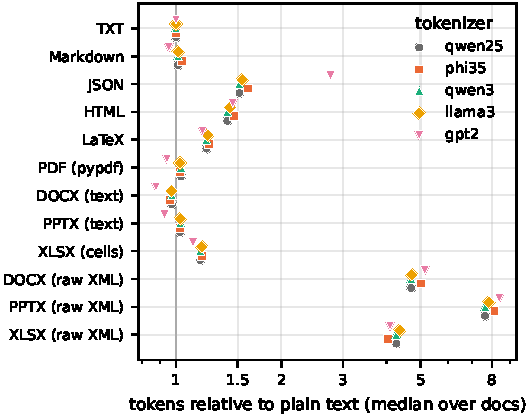
\includegraphics[width=\columnwidth]{figures_full/tokens.pdf}
\caption{Tokens per format relative to the plain-text version of the same
document (median over \NDocs{} documents), under five tokenizers.}
\label{fig:tokens}
\end{figure}

\begin{table}[t]
\centering
\caption{Read cost under the Qwen2.5 tokenizer. Density is
tokens(TXT)/tokens(format). Fixed and per-TXT-token are the intercept and
slope of tokens(format) $= a + b\cdot$tokens(TXT) over the size sweep.
Loader is the time to turn the file into a string.}
\label{tab:overhead}
\resizebox{\columnwidth}{!}{\begin{tabular}{lrrrrr}
\toprule
Format & tokens/TXT & density & loader (ms) & fixed & per TXT tok \\
\midrule
TXT & 1.00 & 100\% & -- & -0 & 1.00 \\
Markdown & 1.01 & 99\% & -- & 4 & 1.01 \\
JSON & 1.52 & 66\% & -- & 73 & 1.41 \\
HTML & 1.40 & 71\% & -- & 200 & 1.10 \\
LaTeX & 1.22 & 82\% & -- & 127 & 1.03 \\
PDF (pypdf) & 1.03 & 97\% & 22.0 & -24 & 1.07 \\
DOCX (text) & 0.97 & 103\% & 8.3 & -18 & 1.00 \\
PPTX (text) & 1.03 & 97\% & 5.6 & -12 & 1.05 \\
XLSX (cells) & 1.17 & 85\% & 3.0 & 64 & 1.08 \\
DOCX (raw XML) & 4.70 & 21\% & 0.2 & 2028 & 1.59 \\
PPTX (raw XML) & 7.65 & 13\% & 0.4 & 1946 & 4.65 \\
XLSX (raw XML) & 4.26 & 23\% & 0.2 & 1276 & 2.30 \\
\bottomrule
\end{tabular}
}
\end{table}

Figure~\ref{fig:tokens} and Table~\ref{tab:overhead} give the read cost.
The formats fall into three groups:
\begin{itemize}
\item \textbf{Extracted text costs what plain text costs.} The text that
  pypdf, python-docx, python-pptx and openpyxl extract is within a few
  percent of TXT. Markdown adds 1\,\%.
\item \textbf{Markup costs 1.2--1.5$\times$.} LaTeX costs
  \TokRatioTex$\times$, HTML \TokRatioHtml$\times$ and JSON
  \TokRatioJson$\times$. The cost model separates them. HTML's overhead is
  mostly fixed (\FixedHtml{} tokens of head and tags; slope
  \SlopeHtml). JSON's grows with content (slope \SlopeJson): every string
  brings quotes, a key and indentation. Under GPT-2's tokenizer, which has
  no tokens for runs of spaces, JSON costs about 2.8$\times$.
\item \textbf{Raw office XML costs 4--8$\times$.} DOCX XML costs
  \TokRatioDocxXml$\times$, XLSX XML \TokRatioXlsxXml$\times$ and PPTX XML
  \TokRatioPptxXml$\times$ (\PptxXmlRatioMin--\PptxXmlRatioMax{} across
  tokenizers). The slide XML's slope is \SlopePptxXml: each word of
  content arrives wrapped in run, paragraph and shape elements.
\end{itemize}
Loading is cheap next to reading: pypdf takes \LoaderPdfText\,ms per
document, while the model's prefill takes about a second.

\subsection{Understand: accuracy}

\begin{figure*}[t]
\centering
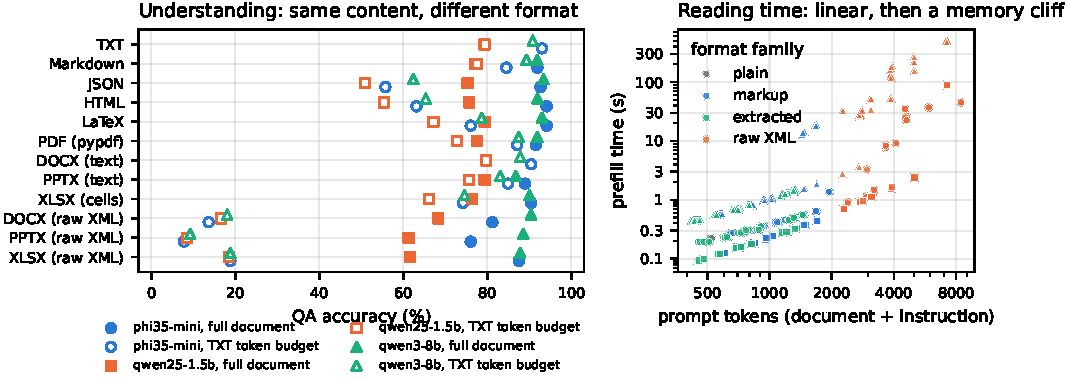
\includegraphics[width=\textwidth]{figures_full/understand.pdf}
\caption{Left: QA accuracy per read format, with the full document
(filled) and with the document cut to its plain-text token count (open).
Right: prefill time against prompt length, one point per
(document, format). Each family of points is linear until the prompt no
longer fits in GPU memory, then rises steeply.}
\label{fig:understand}
\end{figure*}

\begin{table}[t]
\centering
\caption{QA accuracy (\%) with the full document and at the plain-text
token budget, over \NDocs{} documents and about \NQuestionsPerDoc{}
questions each.}
\label{tab:accuracy}
\resizebox{\columnwidth}{!}{\begin{tabular}{lrrrrrr}
\toprule
Format & \multicolumn{2}{c}{phi35-mini} & \multicolumn{2}{c}{qwen25-1.5b} & \multicolumn{2}{c}{qwen3-8b} \\
 & full & budget & full & budget & full & budget \\
\midrule
TXT & 93 & 93 & 79 & 79 & 91 & 91 \\
Markdown & 92 & 85 & 77 & 77 & 92 & 89 \\
JSON & 93 & 56 & 75 & 51 & 93 & 62 \\
HTML & 94 & 63 & 76 & 55 & 92 & 65 \\
LaTeX & 94 & 76 & 79 & 67 & 93 & 79 \\
PDF (pypdf) & 92 & 87 & 77 & 73 & 92 & 87 \\
DOCX (text) & 90 & 90 & 80 & 80 & 88 & 88 \\
PPTX (text) & 89 & 85 & 79 & 76 & 87 & 83 \\
XLSX (cells) & 90 & 74 & 76 & 66 & 90 & 75 \\
DOCX (raw XML) & 81 & 14 & 68 & 17 & 90 & 18 \\
PPTX (raw XML) & 76 & 8 & 61 & 8 & 89 & 9 \\
XLSX (raw XML) & 87 & 19 & 62 & 18 & 88 & 19 \\
\bottomrule
\end{tabular}
}
\end{table}

\paragraph{With the whole document, format barely matters to the larger
model.} Qwen3-8B answers \AccMd\,\% from Markdown and between
\AccPptxText\,\% and \AccJson\,\% from every other format, raw XML
included (Figure~\ref{fig:understand}, Table~\ref{tab:accuracy}). After
Holm correction no format differs from Markdown (smallest adjusted
$p=$\,\MinPVsMd). The smaller models do notice raw XML. Qwen2.5-1.5B drops
from 77\,\% on Markdown to 61--68\,\% on the three XML forms, and
Phi-3.5-mini from 92\,\% to 76--87\,\%, while it scores 89--94\,\% on
every text and extracted form.

\paragraph{At a fixed budget, markup costs answers.} When each format gets
only as many tokens as the plain text, Markdown keeps \AccBudgetMd\,\%.
LaTeX falls to \AccBudgetTex\,\%, HTML to \AccBudgetHtml\,\%, JSON to
\AccBudgetJson\,\%, and raw XML to \AccXmlBudgetMean\,\% on average. Most of
that loss is content that no longer fits. But not all of it: among
questions whose answer string is still inside the cut context, Qwen3-8B
answers \AccBudgetEvidencePlain\,\% from TXT and Markdown and
\AccBudgetEvidenceXml\,\% from raw XML. Markup dilutes the content it does
not push out.

\paragraph{The memory cliff.} Prefill time grows linearly with tokens,
\PrefillMsPerKtok\,ms per thousand tokens for Qwen3-8B ($R^2=$\,\PrefillRsq),
until it doesn't (Figure~\ref{fig:understand}, right). Above
\CliffTokensQwenThreeEightb{} prompt tokens for Qwen3-8B,
\CliffTokensPhiThreeFiveMini{} for Phi-3.5-mini and
\CliffTokensQwenTwoFiveOneFiveb{} for Qwen2.5-1.5B, the time per token
jumps, up to \CliffSlowdown$\times$ the plain-text rate. The GPU has run
out of memory, and the Windows driver spills to system RAM instead of
failing. The one out-of-memory error we hit came from the attention call
asking for 10.8\,GiB at once, which suggests the attention matrix is
materialized in full and grows with the square of the prompt. The prompts past
the cliff are almost all raw XML and JSON. The median raw-PPTX prompt took
\PrefillXmlOverTxt$\times$ as long to read as its TXT version, where the
token ratio alone predicts \TokRatioPptxXml$\times$. The cliff depends on
the stack (GPU memory, attention kernel, driver), but the mechanism is
general: markup moves a document toward whatever memory limit the
hardware has.

\subsection{Write: the format tax}

\begin{figure*}[t]
\centering
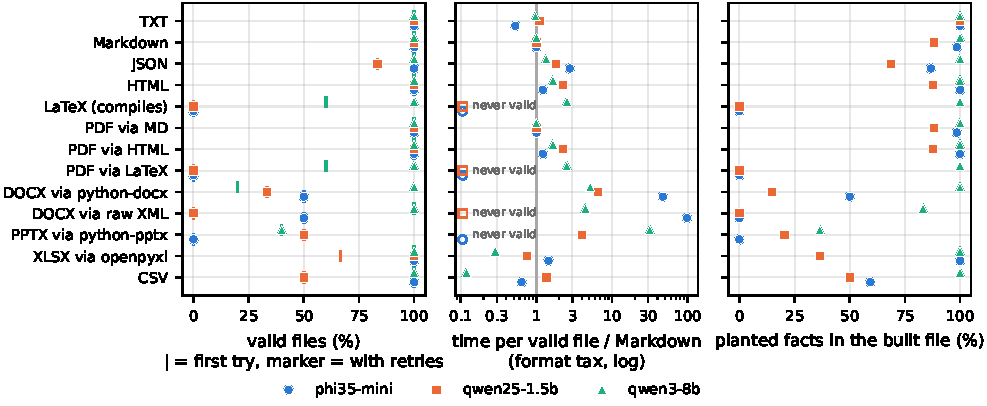
\includegraphics[width=\textwidth]{figures_full/write.pdf}
\caption{Writing each deliverable. Left: share of valid files, after
retries (marker) and on the first try (bar). Middle: time per valid file
relative to Markdown, the format tax (log scale). Right: planted facts that
survive in the built file.}
\label{fig:write}
\end{figure*}

\begin{table*}[t]
\centering
\caption{Writing: valid files (\%), median output tokens over all attempts,
format tax (time per valid file / Markdown) and planted facts recovered
from the built file (\%). Up to \MaxAttempts{} attempts, the build error
fed back each time.}
\label{tab:write}
\resizebox{\textwidth}{!}{\begin{tabular}{lrrrrrrrrrrrr}
\toprule
Deliverable & \multicolumn{4}{c}{phi35-mini} & \multicolumn{4}{c}{qwen25-1.5b} & \multicolumn{4}{c}{qwen3-8b} \\
 & valid & tokens & tax & facts & valid & tokens & tax & facts & valid & tokens & tax & facts \\
\midrule
TXT & 100 & 966 & 0.5 & 100 & 100 & 658 & 1.1 & 100 & 100 & 656 & 1.0 & 100 \\
Markdown & 100 & 1744 & 1.0 & 99 & 100 & 673 & 1.0 & 88 & 100 & 685 & 1.0 & 100 \\
JSON & 100 & 2874 & 2.8 & 87 & 83 & 888 & 1.8 & 69 & 100 & 895 & 1.3 & 100 \\
HTML & 100 & 2118 & 1.2 & 100 & 100 & 1010 & 2.3 & 88 & 100 & 1093 & 1.7 & 100 \\
LaTeX (compiles) & 0 & 6888 & $\infty$ & 0 & 0 & 2112 & $\infty$ & 0 & 100 & 757 & 2.5 & 100 \\
PDF via MD & 100 & 1744 & 1.0 & 99 & 100 & 673 & 1.0 & 88 & 100 & 685 & 1.0 & 100 \\
PDF via HTML & 100 & 2118 & 1.2 & 100 & 100 & 1010 & 2.3 & 88 & 100 & 1093 & 1.7 & 100 \\
PDF via LaTeX & 0 & 6888 & $\infty$ & 0 & 0 & 2112 & $\infty$ & 0 & 100 & 757 & 2.5 & 100 \\
DOCX via python-docx & 50 & 5376 & 47.0 & 50 & 33 & 1210 & 6.5 & 15 & 100 & 2156 & 5.2 & 100 \\
DOCX via raw XML & 50 & 7576 & 98.7 & 0 & 0 & 4016 & $\infty$ & 0 & 100 & 2803 & 4.4 & 83 \\
PPTX via python-pptx & 0 & 6102 & $\infty$ & 0 & 50 & 1250 & 4.0 & 20 & 40 & 5085 & 31.6 & 36 \\
XLSX via openpyxl & 100 & 618 & 1.4 & 100 & 100 & 384 & 0.8 & 36 & 100 & 178 & 0.3 & 100 \\
CSV & 100 & 306 & 0.6 & 59 & 50 & 315 & 1.4 & 50 & 100 & 73 & 0.1 & 100 \\
\bottomrule
\end{tabular}
}
\end{table*}

Figure~\ref{fig:write} and Table~\ref{tab:write} give the cost of each
deliverable. Text formats are cheap and safe: Markdown, TXT, JSON and HTML
were valid for all three models, except one JSON file from the 1.5B
model. Their cost follows their output tokens.

\paragraph{The PDF route decides the PDF's cost.} The same PDF costs
\TaxPdfViaMd$\times$ Markdown through Markdown and xhtml2pdf,
\TaxPdfViaHtml$\times$ through HTML and \TaxPdfViaTex$\times$ through
LaTeX for Qwen3-8B. LaTeX compiled on the first try for only
\FirstValidTex\,\% of documents. Every failure had the same cause: the
table header \emph{Budget (k\$)}, whose unescaped dollar sign opens math
mode. Qwen3-8B
fixed it on retry. Qwen2.5-1.5B and Phi-3.5-mini never did. They resent
the same table every time, so their LaTeX route produced no PDF.

\paragraph{Word through code.} A model writes a .docx only through
python-docx code or raw XML. For Qwen3-8B, python-docx code worked on the
first try for only \FirstValidDocxCode\,\% of documents. It called methods
that do not exist (\texttt{add\_bullet\_list}) or built a table with too
few columns. Retries fixed every case, at a tax of
\TaxDocxCode$\times$. Raw WordprocessingML was valid on the first try every
time, at \TaxDocxXml$\times$. It costs \DocxXmlOverCodeTokens$\times$ the
tokens of the code but needs no repair. It also loses content: only
\RecallDocxXml\,\% of the planted facts survived, against
\RecallDocxCode\,\% for code. The 1.5B model produced no valid raw-XML
document and a valid python-docx file for a third of the documents.
Phi-3.5-mini's one raw-XML file that opened was blank: it put the text
directly inside \texttt{<w:p>}, without the run and text elements Word
displays, so the package is valid and the page is empty. It counts as
valid in Table~\ref{tab:write} and recovers 0\,\% of the facts.

\paragraph{Slides are the most expensive file.} python-pptx decks were
valid for \ValidPptxCode\,\% of documents, at a tax of
\TaxPptxCode$\times$, and Phi-3.5-mini produced none. Phi asked for
placeholders the slide layout does not have
(\texttt{slide.placeholders[1]}). On retry it moved to another missing
index, or kept the same line and added the comment \emph{Corrected line}. The 8B model's typical failure was a script that
defines \texttt{create\_presentation(output\_path)} and never calls it. It
was told, three times, that nothing had been saved. Its decks also carried
only \RecallPptxCode\,\% of the facts: a slide summarizes a paragraph
instead of keeping it.

\paragraph{Spreadsheets are cheap because they are small.} The XLSX and
CSV routes write only the table, so their tax is below 1. Both models
produced valid workbooks every time. The 1.5B model always saved them
under a name of its own choosing instead of the path it was given, and its
workbooks kept only about a third of the table cells.

\paragraph{Retries help only a model that can read the error.} Of
\RetriesQwenTwoFiveOneFiveb{} retries by Qwen2.5-1.5B,
\RetriesFixedQwenTwoFiveOneFiveb{} fixed the file, and
\RetriesSameErrorQwenTwoFiveOneFiveb{} failed again with the identical
error. Qwen3-8B fixed \RetriesFixedQwenThreeEightb{} of
\RetriesQwenThreeEightb, and Phi-3.5-mini \RetriesFixedPhiThreeFiveMini{}
of \RetriesPhiThreeFiveMini. A retry loop multiplies the cost of a route by the
number of attempts. It lowers the cost of a valid file only if the model
can act on the error message.

\subsection{Read and write together}

\begin{figure}[t]
\centering
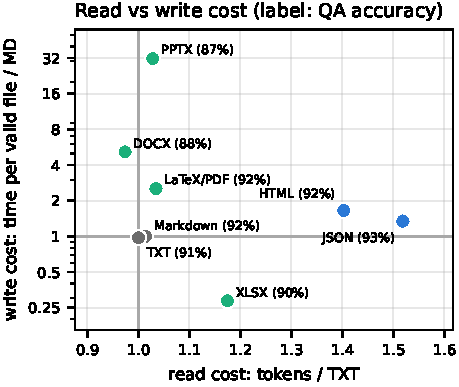
\includegraphics[width=\columnwidth]{figures_full/lifecycle.pdf}
\caption{Each file type for Qwen3-8B: read cost (tokens of its extracted
or marked-up text over TXT) against write cost (format tax). Labels give
full-document QA accuracy.}
\label{fig:lifecycle}
\end{figure}

Figure~\ref{fig:lifecycle} puts the two costs on one plot. Reading and
writing rank the formats differently. DOCX and PPTX are free to read once
their text is extracted, and the most expensive files to write. JSON and
HTML cost about 1.5$\times$ on both axes. Only TXT and Markdown cost about 1 on
both axes, and only Markdown keeps the headings, list and table. A PDF built from Markdown is nearly as cheap.

\section{Discussion}
\label{sec:discussion}

\paragraph{What to send a model.} Extract the text. A PDF, DOCX, PPTX or
XLSX read through a standard loader costs what plain text costs and
answers as well. The loader takes milliseconds. Raw office XML costs
4--8$\times$ the tokens and, at any fixed budget, most of the answers. JSON
and HTML are worth stripping when context is tight: they lose 20--30
points at the plain-text budget. With a large context and a capable
model, format matters little to accuracy. It still matters to time,
memory and money, which all scale with tokens, and on a local GPU
possibly much faster than linearly.

\paragraph{What to ask a model for.} Ask for Markdown, then convert. A PDF
through Markdown cost as much as the Markdown itself. A PDF through LaTeX
cost \TaxPdfViaTex$\times$ for the 8B model and was never produced by the
two smaller models. LaTeX's failures were about escaping, not layout. Office files
are the expensive end. The cost is not in the file but in the code that
makes it, which the model has to get right against a library API, without
seeing the result. A slide deck was the worst case on every measure. An
agent that has to deliver a .docx or .pptx is better served by writing
Markdown and converting it with a fixed, tested tool (pandoc, a template)
than by writing python-docx or python-pptx code each time.

\paragraph{Raw XML is a surprise as an output.} The 8B model never failed
to produce a valid \texttt{document.xml}, while its python-docx code
needed repair in most cases. For a capable model, the format with no API
to misremember was the reliable one. It was not the faithful one, though:
\RecallDocxXml\,\% of the facts against \RecallDocxCode\,\% for code.

\paragraph{Limitations.}
\begin{itemize}
\item \textbf{Small, local models.} The largest model has 8B parameters,
  in 4-bit. Frontier models would fail less, and their tax would shrink
  towards the token ratio. Token counts do not
  depend on model quality. The write results are a lower bound on
  reliability.
\item \textbf{Synthetic documents.} The reports are short (about
  \TxtTokens{} tokens of plain text) and regular. Real office files carry
  styles, revision marks and embedded objects that make raw XML heavier
  than ours, and longer documents would reach the memory cliff sooner.
\item \textbf{Few documents for writing.} Writing used
  \NWriteDocsQwenTwoFiveOneFiveb{} documents for the 1.5B model,
  \NWriteDocsQwenThreeEightb{} for the 8B model (the sixth ran out of
  memory) and \NWriteDocsPhiThreeFiveMini{} for Phi-3.5-mini, which we
  stopped after 7 hours: past the memory cliff, one 8-section document
  would have taken most of a day. Validity rates are coarse at that size, and the tax ratios
  carry the variance of a few slow failures.
\item \textbf{One stack.} The memory cliff belongs to one GPU, one
  attention implementation and one driver. Its position will move with
  all three. Its existence will not, as long as markup adds tokens.
\item \textbf{Fidelity is string recall.} It checks that names and numbers
  survive, not layout, styling or whether a slide reads well.
\end{itemize}

\section{Conclusion}
\label{sec:conclusion}

The format a document arrives in, and the format a model is asked to
produce, carry a cost that is easy to miss because it does not show up
as an error. Reading, the cost is tokens. Markup and raw XML multiply
them, dilute the content at a fixed budget, and on a consumer GPU can tip
a prompt over a memory cliff. Writing, the cost is the pipeline. A PDF,
Word file or slide deck is only ever as cheap as the text, code or XML
the model can get right on the first try.

Markdown is the one format that is cheap to read and cheap to write, and
it converts into a PDF at almost no extra cost. Binary office files are
best read as extracted text. When they must be written, a model's code is
the expensive part: a fixed converter is cheaper.


\FloatBarrier
\bibliographystyle{plain}
\bibliography{references}
\end{document}
